\documentclass[14pt,fleqn]{extarticle}
\RequirePackage{prepwell}
\previewoff
\begin{document}

\newcommand\ptp{ \left(x_p,y_p \right)}
\newcommand\xp{x_P}
\newcommand\xps{{\xp}^2}

%text
Find the equation of the normal at a point
on the curve $x^2=4y$ which passes
through the point $(1,2)$. Also, find the
equation of the corresponding tangent
%

\newcard 

In $x^2 = 4y$, notice that $y \geq 0$ for all $x$. Hence, the curve is an upward facing parabola \newline 

The point $A = \left(1,2 \right)$ \underline{does not} lie on the parabola $\left(1^2 \neq 4\cdot 2 \right)$ \newline 

But some line $N$ passes through $A$ such that $N$ is the normal at a point $P$ on the parabola -- a shown in the figure below \newline 

We have to find both $N$ and $T$ (the tangent at $P$) 

\begin{center}
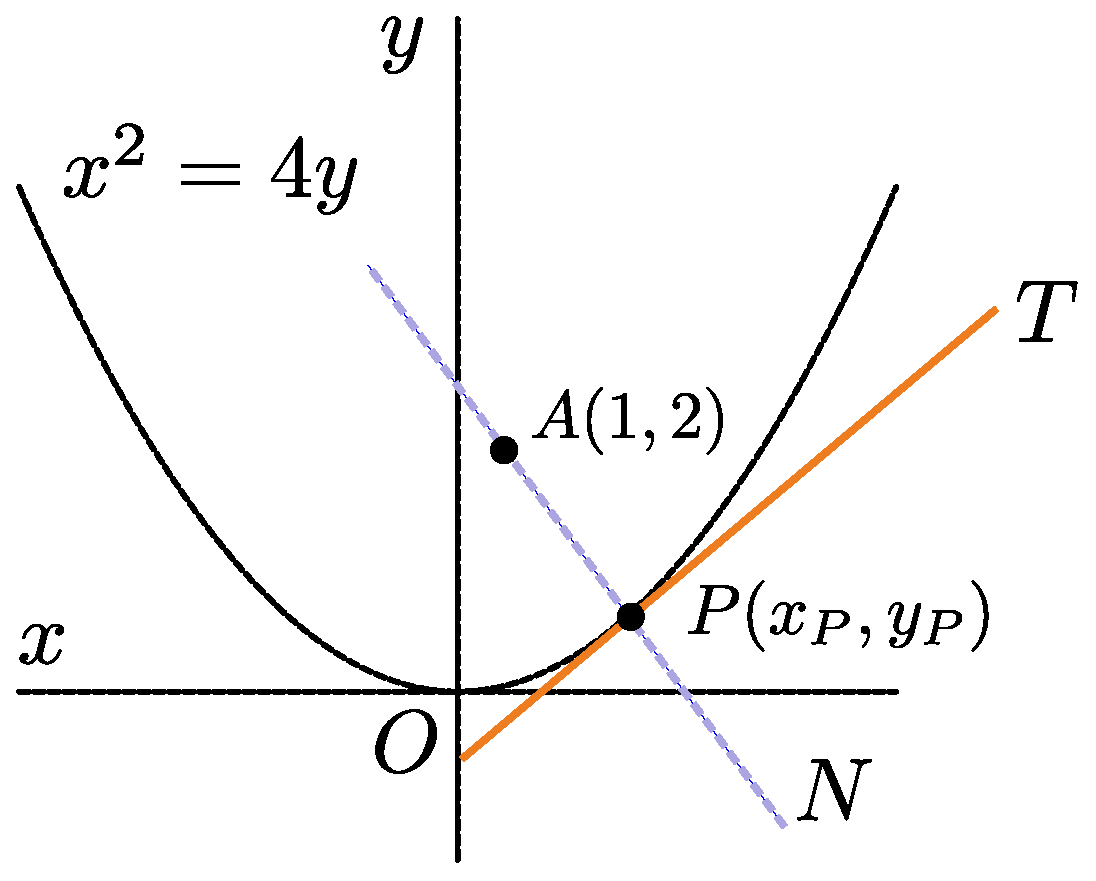
\includegraphics[scale=0.35]{fig-1.eps} 
\end{center}

\newcard

At point $P = \ptp$ where the normal $N$ intersects the parabola 
\begin{align}
m_T &= \frac{x_p}{2}\text{ and } \frac{y_p-2}{x_p-1} = -\frac{2}{x_p}
\end{align}

where $m_T$ is the slope of the tangent $T$ at point $P$ 

\newcard 

At point $P = \ptp$ where the normal $N$ intersects the parabola 
\begin{align}
m_T &= \frac{x_p}{2}\text{ and } \frac{y_p-1}{x_p-2} = \frac{2}{x_p} 
\end{align}

where $m_T$ is the slope of the tangent $T$ at point $P$ 

\newcard 

For any point $P=\ptp$ on the parabola 
\begin{align}
m_T &= \frac{dy}{dx} = \frac{d}{dx}\left( \frac{x^2}{4}\right) = \frac{x}{2} \\
\therefore m_N &= -\frac{1}{m_T} = -\frac{2}{x}
\end{align}

But the normal $N$ also passes through $A$

\begin{align}
\therefore m_N &= \frac{y_P - 2}{x_p - 1} = -\frac{2}{x_P}
\end{align}

\newcard 
$P = \left( 2,1\right)$ 

\newcard 

$P = \left(3,1 \right)$

\newcard 
We know that 
\begin{align}
	\frac{y_P - 2}{x_P - 1} = -\frac{2}{x_P} &\text{ and } \underbrace{y_P = \frac{{x_P}^2}{4}}_{\text{$P$ is on the parabola}} \\
	\therefore \frac{\frac{\xps}{4} - 2}{x_P - 1} &= -\frac{2}{x_P} \\
	\text{or } \xp\cdot \left(\xps - 8 \right) &= -8\cdot \left(\xp-1 \right) \\
	\implies {\xp}^3 - 8\xp &= -8\xp + 8 \\
	\implies {\xp}^3 &= 8\text{ or }\xp = 2  \\
	\therefore y_P &= \frac{\xps}{4} =  1 
\end{align}

Hence, $P = (2,1)$ 

\newcard 

The equations of the normal and the tangent are therefore 
\begin{align}
	N&: x+y = 3 \\
	T&: y = x - 1 
\end{align}

\newcard 

The equations of the normal and the tangent are therefore 
\begin{align}
	N&: x+y = 1 \\
	T&: y = x - 3 
\end{align}

\newcard 

Both the tangent and the normal pass through $P=(2,1)$. But they have different slopes -- which we also know how to find 

\begin{center}
  \begin{tabular}{NNN}
   \toprule
        \text{Line} & \text{Slope} & \text{Equation} \\
   \midrule 
   N & -\frac{2}{\xp} = -1 & \frac{y - 1}{x -2 } = -1 \\
   & & \implies x + y = 3 \\
    \midrule 
    T & \frac{2}{\xp} = 1 & \frac{y-1}{x-2} = 1 \\
    & & \implies y = x - 1 \\
    \bottomrule
  \end{tabular}
\end{center}

\end{document}